% Bloque final DQN: cifras y gráficas regeneradas desde el mismo cache.
% Generado desde figuras/dqn_resultados.json.
\newcommand{\DQNExperiencias}{2400}
\newcommand{\DQNActualizaciones}{2337}
\newcommand{\DQNSincronizaciones}{19}
\newcommand{\DQNAccion}{HOLD}
\newcommand{\DQNRecompensa}{0.00}
\newcommand{\DQNPredict}{580.44}
\newcommand{\DQNMaxFuturo}{585.64}
\newcommand{\DQNTarget}{579.79}
\newcommand{\DQNHube}{0.216}
\newcommand{\DQNEpsilon}{0.05}
\newcommand{\DQNValidacionA}{+1.49}
\newcommand{\DQNValidacionB}{+1.49}
\newcommand{\DQNDecisionTest}{BUY\_POL}
\newcommand{\DQNQBuy}{867.24}
\newcommand{\DQNQHold}{591.55}
\newcommand{\DQNTestInicio}{22-Aug 18:00}
\newcommand{\DQNTestFin}{22-Aug 22:00}
\newcommand{\DQNTestRetDQN}{-4.12}
\newcommand{\DQNTestDrawDQN}{-4.12}
\newcommand{\DQNTestRetQ}{-4.40}
\newcommand{\DQNTestDrawQ}{-4.40}
\newcommand{\DQNTestRetBellman}{-4.12}
\newcommand{\DQNTestDrawBellman}{-4.12}
\newcommand{\DQNTestRetHold}{-4.12}
\newcommand{\DQNTestDrawHold}{-4.12}

% Generado desde figuras/replay_comun_pol.json.
\newcommand{\DQNReplayHoras}{23}
\newcommand{\DQNReplayInicio}{22-Aug 02:00}
\newcommand{\DQNReplayFin}{23-Aug 01:00}

% Generado con el registro del experimento DQN.
\newcommand{\DQNTrainDecisiones}{2400}
\newcommand{\DQNTestDecisiones}{4}
\newcommand{\DQNTrainExploracion}{46.0}
\newcommand{\DQNTrainTransiciones}{1800}
\newcommand{\DQNTestTransiciones}{3}
\newcommand{\DQNPrimerEstado}{DOWN/HOLD/USDC}
\newcommand{\DQNPrimerSiguiente}{DOWN/HOLD/POL}
\newcommand{\DQNPrimerAccion}{BUY\_POL}
\newcommand{\DQNPrimerQ}{269.4}
\newcommand{\DQNPrimerQAlternativa}{128.7}


\begin{frame}{DQN: el mismo problema POL con una red de valores}
\begin{block}{Continuidad del problema}
\small Decisiones horarias en POL/USDC; estado con mercado, wallets y posición; acciones Buy, Sell y Hold admisibles; recompensa económica neta de gas y ajuste por wallets.
\end{block}
\vspace{.6em}
\begin{columns}[c,onlytextwidth]
\column{.23\textwidth}\centering\colorbox{lightpanel}{\parbox[c][1.4cm][c]{.92\linewidth}{\centering\textbf{Estado}\\[.3em]9 entradas}}
\column{.03\textwidth}\centering$\rightarrow$
\column{.21\textwidth}\centering\colorbox{lightpanel}{\parbox[c][1.4cm][c]{.92\linewidth}{\centering\textbf{Capa 1}\\[.3em]32 + ReLU}}
\column{.03\textwidth}\centering$\rightarrow$
\column{.21\textwidth}\centering\colorbox{lightpanel}{\parbox[c][1.4cm][c]{.92\linewidth}{\centering\textbf{Capa 2}\\[.3em]32 + ReLU}}
\column{.03\textwidth}\centering$\rightarrow$
\column{.22\textwidth}\centering\colorbox{lightpanel}{\parbox[c][1.4cm][c]{.92\linewidth}{\centering\textbf{Salida}\\[.3em]3 valores Q}}
\end{columns}
\vspace{.7em}
\small
\begin{itemize}
\item Entradas: régimen (3), señal de wallets (4), posición (1) y etapa normalizada (1).
\item La posición limita las acciones: en USDC, Buy/Hold; en POL, Sell/Hold.
\item Cada salida estima una recompensa acumulada descontada; no es una probabilidad.
\end{itemize}
\end{frame}

\begin{frame}{Cómo aprende la red DQN}
\begin{block}{Una experiencia}
\centering $(x_t,a_t,r_{t+1},x_{t+1},done)$ se guarda en el \emph{replay buffer}.
\end{block}
\begin{columns}[T,onlytextwidth]
\column{.50\textwidth}
\begin{enumerate}\small
\item $\varepsilon$-greedy explora o elige el mayor Q admisible.
\item Se extrae un minilote de 64 experiencias.
\item Huber compara $Q_\theta(x_t,a_t)$ con el objetivo.
\item Adam ajusta la red principal; la red objetivo se sincroniza cada 120 actualizaciones.
\end{enumerate}
\column{.47\textwidth}
\begin{block}{Objetivo de Bellman}
\[
y_t=r_{t+1}+\gamma(1-done)
\max_{a'\in A(x')}Q_{\theta^-}(x_{t+1},a')
\]
\small $\gamma=0.99$. El máximo excluye acciones inadmisibles. Si $done=1$, $y_t=r_{t+1}$.
\end{block}
\end{columns}
\end{frame}

\begin{frame}{Entrenamiento DQN: recompensa y pérdida}
\centering
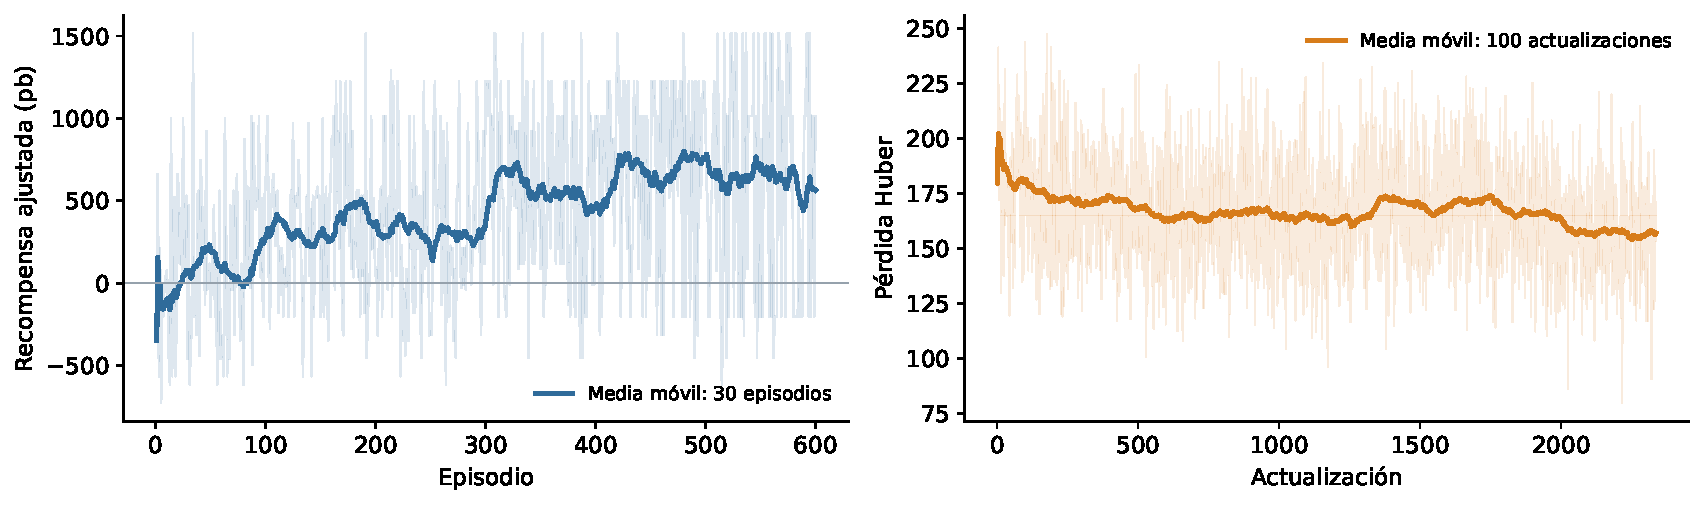
\includegraphics[width=.98\textwidth,height=.55\textheight,keepaspectratio]{dqn_entrenamiento}
\begin{itemize}\small
\item \DQNExperiencias{} experiencias; \DQNActualizaciones{} actualizaciones; \DQNSincronizaciones{} sincronizaciones.
\item La recompensa mostrada incluye el ajuste por wallets; Huber mide error frente al target.
\item Ambas curvas describen entrenamiento, no demuestran rentabilidad futura.
\end{itemize}
\end{frame}

\begin{frame}{Auditoría: una transición del replay buffer}
\begin{columns}[T,onlytextwidth]
\column{.49\textwidth}
\begin{block}{Datos de la experiencia}
\small
\begin{tabular}{lr}
\toprule
Componente & Valor \\
\midrule
Acción ejecutada & \DQNAccion \\
Recompensa inmediata & \DQNRecompensa{} pb \\
Fin del episodio & No \\
$Q_\theta(x_t,a_t)$ & \DQNPredict{} pb \\
Máximo Q futuro admisible & \DQNMaxFuturo{} pb \\
\bottomrule
\end{tabular}
\end{block}
\column{.48\textwidth}
\begin{block}{Cálculo}
\small
\[
y=\DQNRecompensa+0.99(\DQNMaxFuturo)
\]
\[
\boxed{y=\DQNTarget\ \text{pb}}
\]
\centering Pérdida de Huber: \DQNHube.
\end{block}
\end{columns}
\vspace{.5em}
\small Valores calculados con los pesos al finalizar el entrenamiento; la transición fue guardada en train.
\end{frame}


\begin{frame}{¿Qué acciones tomó el DQN en train y test?}
\centering
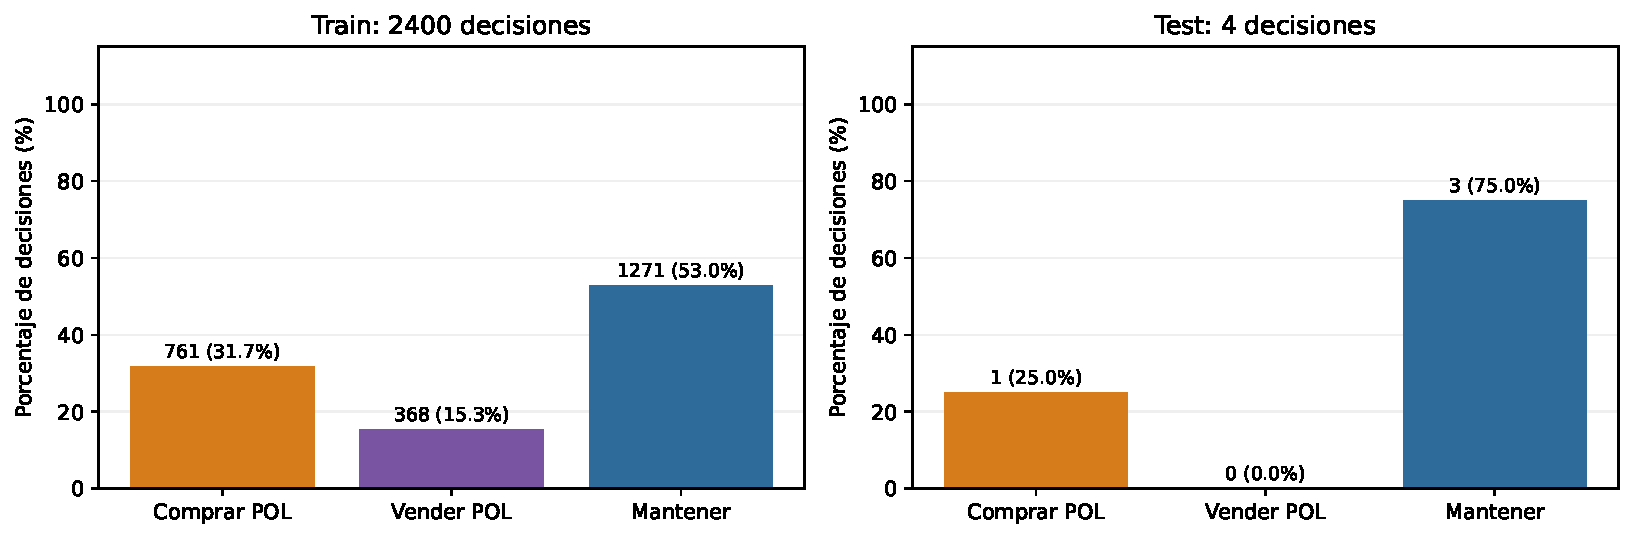
\includegraphics[width=.94\textwidth,height=.52\textheight,keepaspectratio]{dqn_acciones_train_test}
\begin{itemize}\small
\item Train: \DQNTrainDecisiones{} decisiones de episodios repetidos; \DQNTrainExploracion\% elegidas por exploración.
\item Test: \DQNTestDecisiones{} decisiones con la red congelada y sin exploración; muestra muy corta.
\item En USDC solo puede comprar o mantener; en POL, vender o mantener.
\end{itemize}
\end{frame}

\begin{frame}{¿Cómo cambian los estados?}
\centering
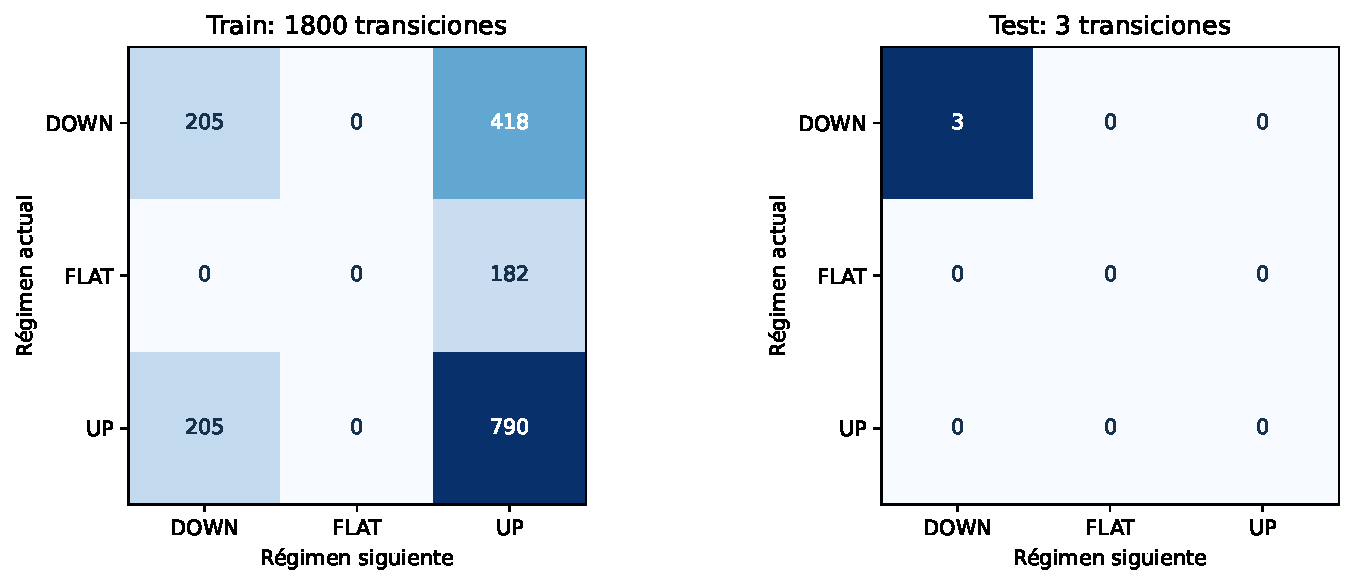
\includegraphics[width=.88\textwidth,height=.49\textheight,keepaspectratio]{dqn_transiciones_train_test}
\begin{itemize}\small
\item Filas: régimen actual; columnas: siguiente. Train: \DQNTrainTransiciones{} transiciones; test: \DQNTestTransiciones{}.
\item El estado completo incluye régimen, wallets, posición y etapa; el gráfico resume solo el régimen.
\item Test: \DQNPrimerEstado{} $\xrightarrow{\text{\DQNPrimerAccion}}$ \DQNPrimerSiguiente. El último paso es terminal.
\item Las escalas de color son independientes; el mercado siguiente no lo controla el agente.
\end{itemize}
\end{frame}

\begin{frame}{Replay histórico común: cuatro políticas sobre POL}
\centering
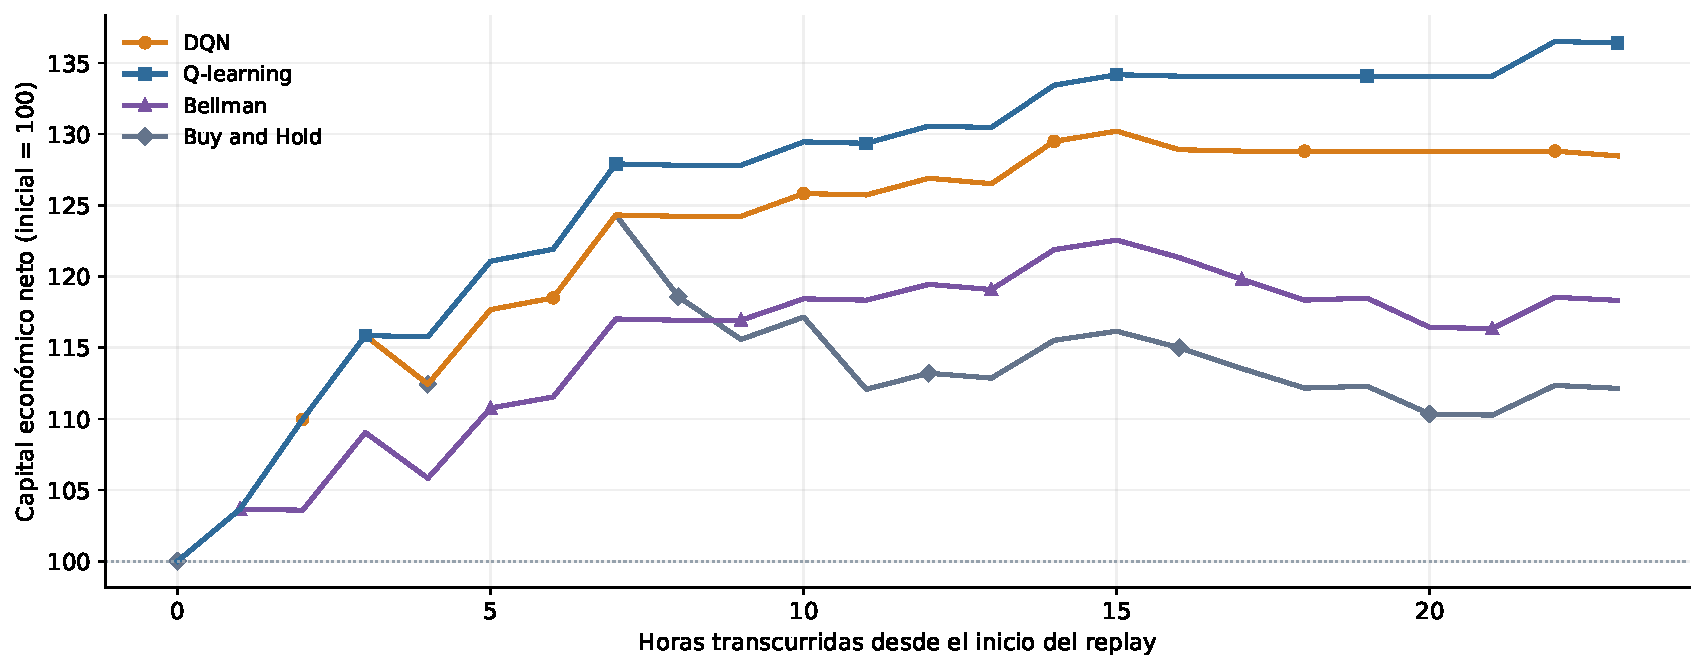
\includegraphics[width=.98\textwidth,height=.59\textheight,keepaspectratio]{replay_comun_pol}
\begin{itemize}\small
\item \DQNReplayHoras{} horas completas: \DQNReplayInicio{} a \DQNReplayFin{} UTC; capital inicial 100.
\item Los cuatro recorridos usan el mismo precio y contabilidad; la posición se mantiene entre horas.
\item Modelos entrenados en este período: replay \textbf{dentro de muestra}. Test reservado: ver anexo.
\item La última hora incompleta se excluye; curvas con el mismo capital se superponen.
\end{itemize}
\end{frame}

\begin{frame}{Sensibilidad: retirar la señal de wallets}
\centering
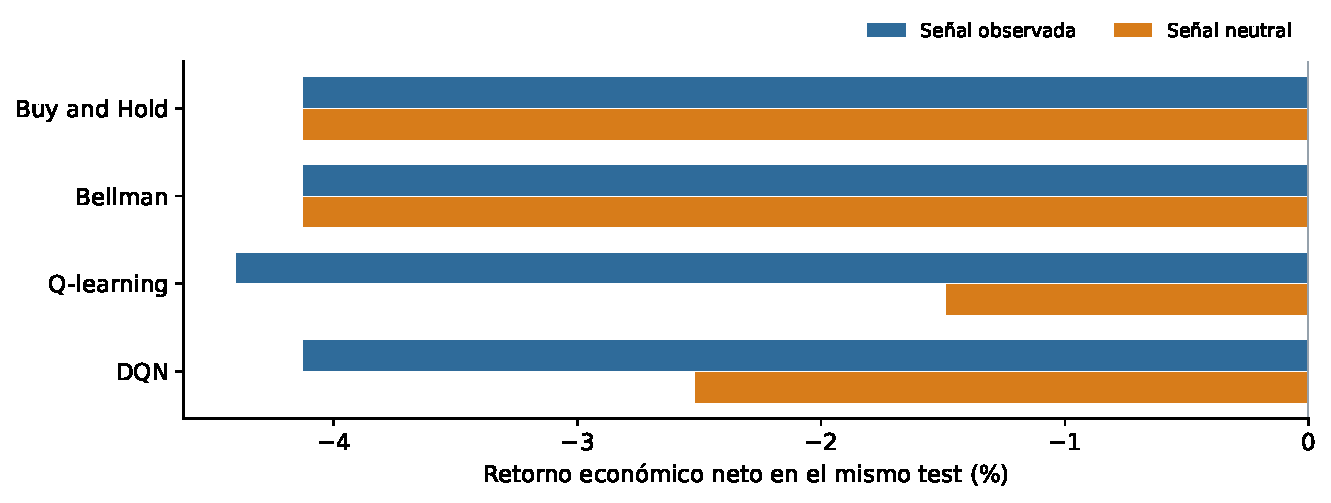
\includegraphics[width=.88\textwidth,height=.55\textheight,keepaspectratio]{dqn_estres}
\begin{itemize}\small
\item En el mismo test sustituimos la señal y los apoyos por neutral, sin reentrenar.
\item El resultado muestra sensibilidad a una intervención; no es otro test independiente.
\item Cambio DQN: $\varepsilon_{\mathrm{final}}=0.05$ y $0.30$ obtuvieron \DQNValidacionA\% y \DQNValidacionB\% en validación; se eligió \DQNEpsilon{} por desempate.
\end{itemize}
\end{frame}

\begin{frame}{Limitaciones y pasos siguientes}
\begin{columns}[T,onlytextwidth]
\column{.48\textwidth}
\begin{block}{Datos y evaluación}
\small Un solo snapshot cercano a 24 horas. Train, validación y test usan bloques de 4 horas; el test es demasiado corto para inferir desempeño futuro. Faltan auditoría temporal del ledger, slippage y profundidad.
\end{block}
\column{.48\textwidth}
\begin{block}{Modelos}
\small Bellman depende de transiciones escasas; Q tabular tiene estados sin visitas; DQN puede sobreajustar y generalizar mal. La pérdida Huber no equivale a rentabilidad.
\end{block}
\end{columns}
\vspace{.5em}
\begin{alertblock}{Siguiente comprobación}
\small Ampliar snapshots, construir períodos independientes de 24 horas y repetir validación temporal sin ajustar al test.
\end{alertblock}
\end{frame}
